To be able to find anomalies and outliers we will in this section, use some different methods to be able find the most likely anomalies and outliers. Afterwards we will then compare the different methods we have done on our data, to get the most likely outliers from the different methods we have used.

Using leave-one-out, we were able to find the optimal kernel width to $0.25$.

\subsection{Density Estimation}

When are checking our different data objects estimated density, we do not want our data to be in an low density area, since they then most likely would be outliers.

When we look at a Gaussian density estimation of all our data objects we can actual see that we properly have below a 100 outliers, which we then afterwards only takes a look at those 100. Here we see that around the 20 outliers it starts to grow, which means we can take a look at those, and when we closer to those we see around the 17-19 that it have an significant growth which could mean that we have some outliers lying below these, it should be said the some these might not be outliers.

\begin{figure}[H]
\centering
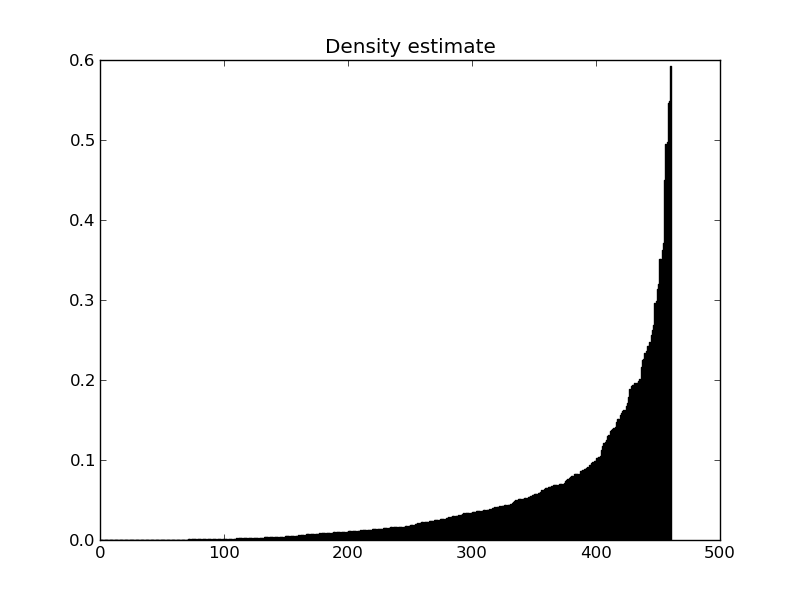
\includegraphics[width=5cm, keepaspectratio=true]{pictures/densityEstimationAll.png}
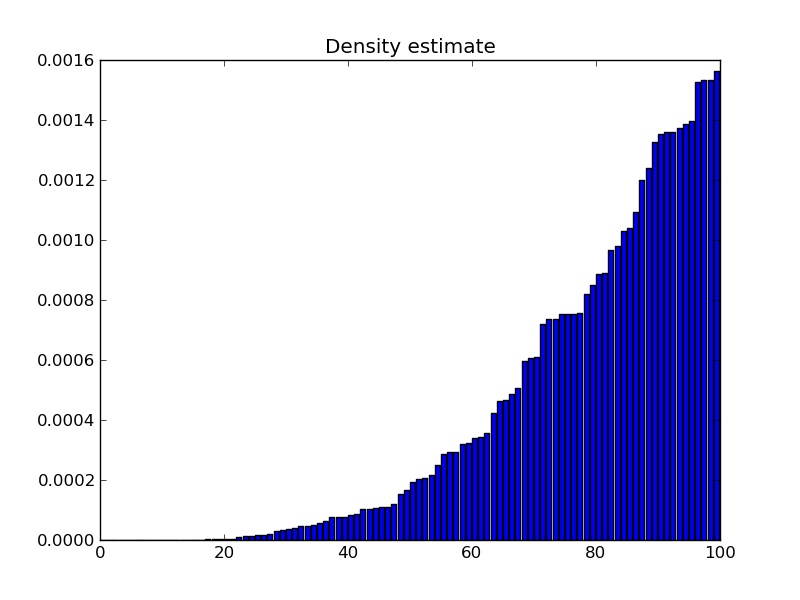
\includegraphics[width=5cm, keepaspectratio=true]{pictures/densityEstimation100.png}
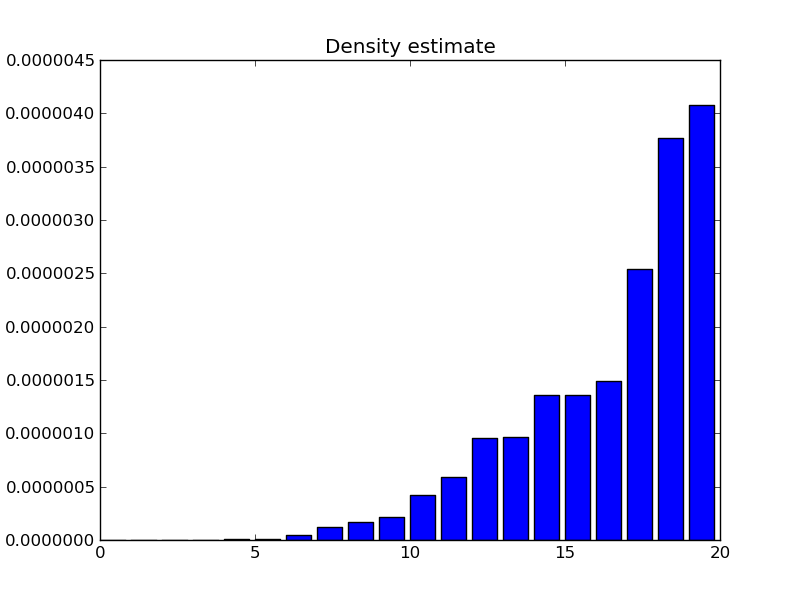
\includegraphics[width=5cm, keepaspectratio=true]{pictures/densityEstimation20.png}
\vspace{-0.4cm}
\caption{\footnotesize Outlier score gaussian density estimation}
\label{gkd}
\end{figure}

With a KNN density estimation we want to have some of the same data object as with gassian density estimation to be in the low density end. So we are able to confirm that we have some outliers. As with the Gaussian method, we again first look at figure of all the data objects, which shows a bit better then Gaussian where we have a sudden increase of density. In this case its already starts in the first data object and increase drastic until around the 50 data object. So after this we take a look at 100 lowest density scores, this actual shows that we have the most drastic increase around the 5'th lowest density data objects, but to have bit more data to look at we now look at 20 lowest density. This show that the 4 lowest densities most likely is outliers.

\begin{figure}[H]
\centering
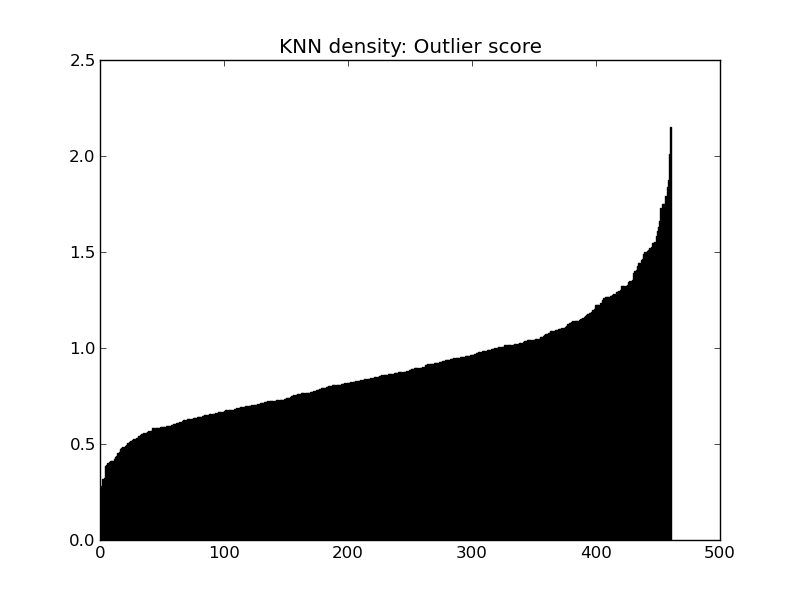
\includegraphics[width=5cm, keepaspectratio=true]{pictures/knndensityEstimationAll.png}
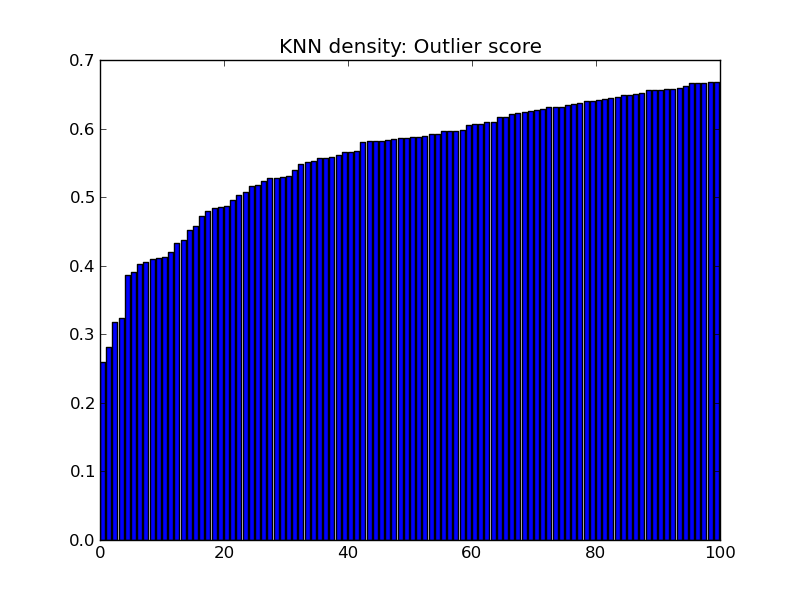
\includegraphics[width=5cm, keepaspectratio=true]{pictures/knndensityEstimation100.png}
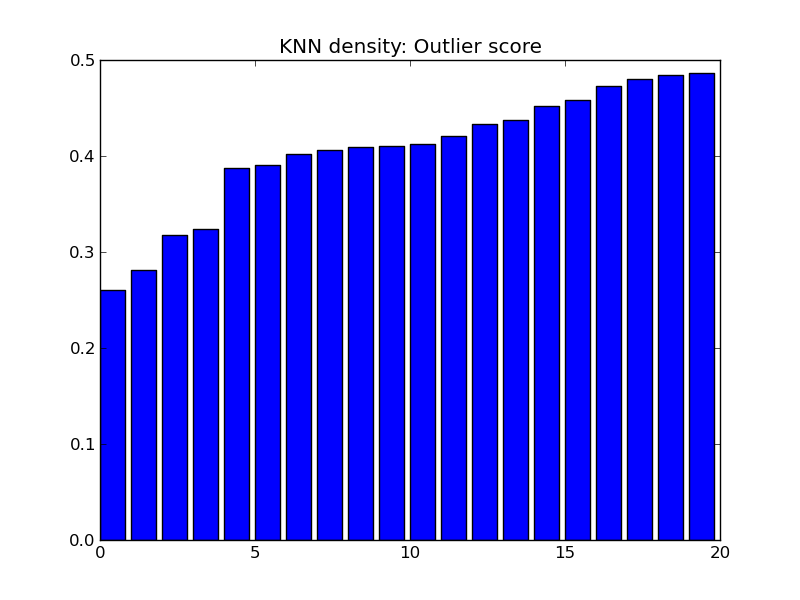
\includegraphics[width=5cm, keepaspectratio=true]{pictures/knndensityEstimation20.png}
\vspace{-0.4cm}
\caption{\footnotesize Outlier score knn density estimation}
\label{knn}
\end{figure}

As with Gaussian and KNN we start with to look at all the data objects score, and see it increases quick in the beginning, so we take a look at the 20 lowest data objects. In this graph we the see that the from the data object with the lowest density to the next one we have the biggest jump in density, which most likely would make the data object with the lowest density an outlier.

\begin{figure}[H]
\centering
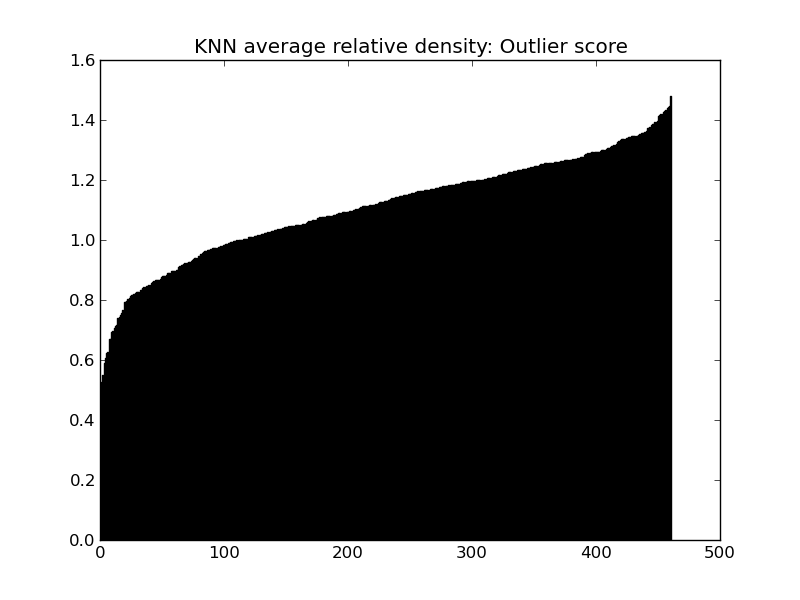
\includegraphics[width=7.5cm, keepaspectratio=true]{pictures/knnAvgdensityEstimationAll.png}
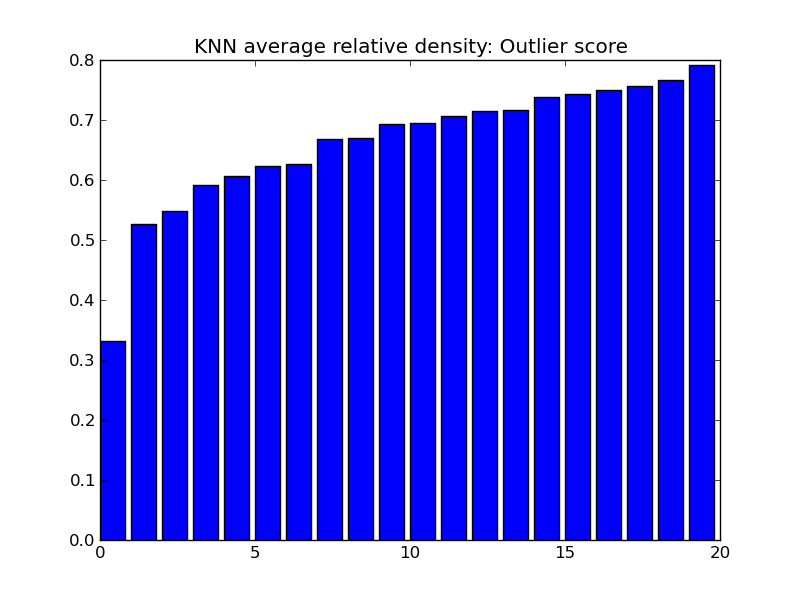
\includegraphics[width=7.5cm, keepaspectratio=true]{pictures/knnAvgdensityEstimation20.png}
\vspace{-0.4cm}
\caption{\footnotesize Outlier score knn average relative density estimation}
\label{avg}
\end{figure}

\subsection{KNN Distance}

When we take a look at the distance method, we see that this time we go from best score to worst score, but it show about the same as the density methods. That it around the numbers of high outlier score as with the density as well as low outlier scores, which can be seen in the table below. You can also see that it is some of the same data objects that keeps showing up in all the different runs, that can be seen in the table below.

\begin{table}[H]
\begin{longtable}{lccccc}
\hline
   & 1   & 2   & 3   & 4   & 5   \\ \hline
5  & 21  & 345 & 362 & 426 & 442 \\ 
10 & 345 & 21  & 362 & 426 & 8   \\ 
25 & 345 & 362 & 21  & 426 & 241 \\
50 & 345 & 362 & 241 & 21  & 359 \\ \hline
\end{longtable}
\end{table}


\subsection{Comparison of outlier score}

When we compare the different outlier score and see which data objects the different methods found, we see that some of them are recurring. If we look at the first data object in all 4 methods, we see that the first have 345 but is in 2 row for the last data object, this properly means that this is an outlier since each method gave it a bad score. If we then take a look at some of the others we see that some of them is recurring in at least one of the other methods, this could mean that these is outliers to. If we take a look at the table below we can properly say that data object 345, 246, 362, 241 and 442 is outliers because of they have a low score and is recurring in at least one of the other methods.


\begin{table}[H]
\begin{longtable}{lcccc}
\hline
  & Gaussian & KNN & AVG KNN & Dist \\ \hline
1 & 345      & 345 & 345     & 21 \\ 
2 & 426      & 426 & 140     & 345 \\ 
3 & 362      & 362 & 141     & 362 \\ 
4 & 241      & 442 & 426     & 426 \\ 
5 & 334      & 241 & 39      & 442 \\ \hline
\end{longtable}
\end{table}
